\documentclass[11pt]{article}
\usepackage[margin=1in]{geometry}
\usepackage{volfit_preamble}
\graphicspath{{figures/}}

\title{\textbf{One Number, Three Integrals}\\[2pt]
\large The variance swap as a linear functional, and the representation
where each model finds it cheap\\[2pt]
\normalsize Vol-Fitter Technical Notes, No.~08}
\author{Vol-Fitter}
\date{\today}

% Note-local notation (shared symbols come from volfit_preamble).
\newcommand{\wvs}{w_{\mathrm{vs}}}
\newcommand{\svs}{\sigma_{\mathrm{vs}}}
\newcommand{\lam}{\lambda}
\newcommand{\Lo}{\Lambda}

\begin{document}
\maketitle

% Generated numbers.  vs_repr_tables.tex carries everything unique to this
% edition (gen_vs_representations.py).  Never retype a generated number.
% Auto-generated by gen_vs_representations.py — do not edit.
\newcommand{\vsrclosed}{24.47}
\newcommand{\vsrrepl}{24.49}
\newcommand{\vsragreebp}{1.53}
\newcommand{\vsrlvvol}{24.17}
\newcommand{\vsrlvgapbp}{30}
\newcommand{\vsrwingsharepct}{13}
\newcommand{\vsratmsharepct}{48}
\newcommand{\vsrtruncsixbp}{0.007}
\newcommand{\vsrtruncplateau}{2.2}
\newcommand{\vsrprodeightbp}{2.72}
\newcommand{\vsrreplfinebp}{0.06}
\newcommand{\vsrlvbellybp}{13}
\newcommand{\vsrlvwingpts}{3.6}
\newcommand{\vsrbasefitbp}{0.2}
\newcommand{\vsrtarget}{25.97}
\newcommand{\vsrpulled}{25.75}
\newcommand{\vsrpullsharepct}{85}
\newcommand{\vsrpullfitbp}{52}
\newcommand{\vsrsensabs}{\ensuremath{1.2\times10^{-10}}}
\newcommand{\vsrsensrel}{\ensuremath{1.7\times10^{-6}}}
\newcommand{\vsrsenslive}{19}
\newcommand{\vsrsenstotal}{21}
\newcommand{\vsrlvagreebp}{0.78}
\newcommand{\vsrheroagreebp}{0.00}
\newcommand{\vsrherospreadbp}{717}
\newcommand{\vsrheronodes}{6}
\newcommand{\vsrrefagree}{-17}
\newcommand{\vsrhalfwidth}{6}
\newcommand{\vsrpoints}{801}
\newcommand{\vsrgencommit}{b20cadd}
\newcommand{\vsrgendate}{2026-07-18}


\begin{abstract}
Fit two production models --- a parametric slice and a local-volatility
surface --- to the same twenty-three option quotes and they agree to basis
points at every quoted strike; yet their fair variance-swap strikes differ
by \vsrlvgapbp\ vol bp, because the fair strike is a \emph{global}
functional of the smile, and the quotes leave its wing share free.  A
variance-swap quote is therefore genuinely new information: one number per
$(\text{underlying},T)$ node that pins what scattered option quotes cannot.
This lecture develops that number as a single pairing --- the log-contract
payoff integrated against the terminal risk-neutral law --- and shows that
the pairing has \emph{three} exact integral representations: against option
prices across strikes (Carr--Madan), against the quantile function of the
terminal law, and against the local-variance field along paths
(a source PDE).  All three are the same number; what differs is the cost of
evaluation in each model's native coordinates, and the first production
wiring --- one uniform replication for every model --- turned a millisecond
fit into a measured $158$-second one because it evaluated the pairing in a
chart where every point is a root-find.  The per-model routes that replaced
it are audited here end to end: the quantile-side closed form agrees with
the strike-side replication to \vsragreebp\ vol bp on the running slice
(and the gap is \emph{spacing}, not truncation: tails beyond the
half-width contribute \vsrtruncsixbp\ bp while the production grid's
trapezoid carries \vsrreplfinebp--\vsragreebp\ bp of $O(\Delta k^2)$
error); the source PDE matches its own strike-side value to
\vsrlvagreebp\ variance bp with analytic parameter sensitivities equal to
finite differences at \vsrsensabs; and the closed form re-derives the six
fair strikes published by the application for a real SPY surface to
\vsrheroagreebp\ vol bp.  As a calibration target the quote enters as one
extra residual in volatility units, weighted as a fraction (default ten
percent) of the node's option weight; at the default it moves a smile whose
natural fair strike is \vsrclosed\% to \vsrpulled\% against a
\vsrtarget\% quote --- \vsrpullsharepct\% of the way --- at a worst
option-quote concession of \vsrpullfitbp\ vol bp.
\end{abstract}

\newpage
\tableofcontents
\newpage

%======================================================================
\section{The number the quotes leave free}
\label{sec:free}

Start with the failure the machinery exists to prevent.
\Cref{fig:ident} shows two fits to one quote set: the parametric slice
this series calls LQD (Note~01) and the piecewise-affine local-volatility
surface (Note~04), both production calibrations, both threading the same
twenty-three quotes --- inside the quoted band the two implied-volatility
curves are within \vsrlvbellybp\ vol bp of each other.  Outside it they
separate by up to \vsrlvwingpts\ vol \emph{points}, and their fair
variance-swap strikes --- \vsrclosed\% and \vsrlvvol\% --- differ by
\vsrlvgapbp\ vol bp.  Nothing has gone wrong: both models price every
quote correctly, and the data simply does not decide the quantity.  A
desk that marks variance swaps, or hedges wing risk, needs that quantity
decided.

\begin{figure}[H]
\centering
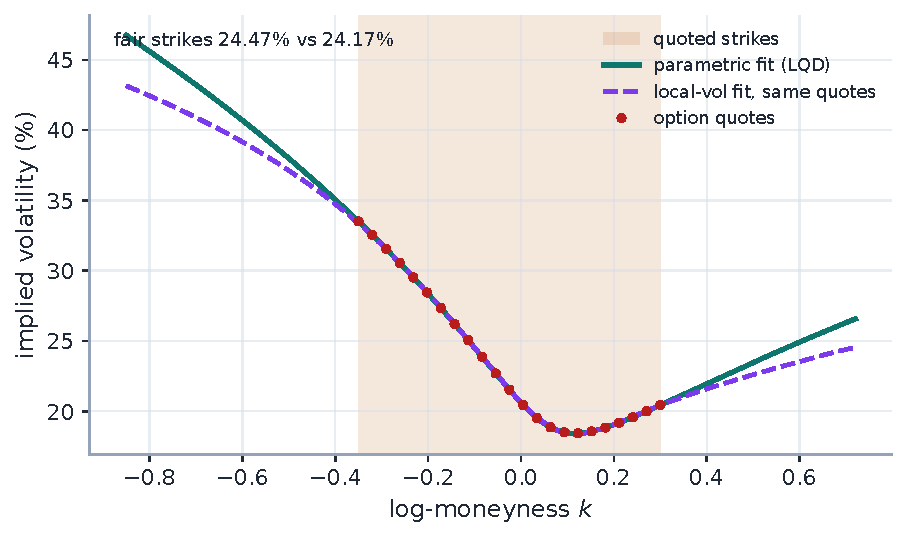
\includegraphics[width=0.86\textwidth]{fig_vsr_ident.pdf}
\caption{The identifiability gap, exhibited with two production models on
one quote set.  Inside the quoted band (shaded) the parametric and
local-vol fits agree to \vsrlvbellybp\ vol bp --- the quotes pin both.
Outside it they diverge by up to \vsrlvwingpts\ vol points, and the fair
var-swap strikes printed by the two models differ by \vsrlvgapbp\ vol bp.
The fair strike is a global functional; option quotes constrain it only
through the belly.}
\label{fig:ident}
\end{figure}

\subsection{The instrument, and the functional it prices}

A variance swap pays the realized variance of the underlying up to $T$
against a fixed strike.  Work throughout in forward-normalized units: the
underlying is quoted as a ratio of the forward for $T$, so $F=1$, strikes
are $K=e^{k}$ with $k$ the log-moneyness, and $X=\log S_T$ is the terminal
log-return.  Under a continuous forward-measure diffusion
$\dd S_t/S_t=\sigma_t\,\dd W_t$, It\^o's formula applied to $\log S_t$
gives
\begin{equation}
\dd \log S_t=\frac{\dd S_t}{S_t}-\half\sigma_t^2\,\dd t
\qquad\Longrightarrow\qquad
\int_0^T\!\sigma_t^2\,\dd t
=2\!\int_0^T\!\frac{\dd S_t}{S_t}-2\log S_T .
\label{eq:ito}
\end{equation}
The stochastic integral is a martingale, so taking forward-measure
expectations kills it, and the fair strike --- the expected total
variance --- is the expectation of a fixed \emph{payoff}:
\begin{equation}
\wvs=\E\!\Big[\int_0^T\!\sigma_t^2\,\dd t\Big]=\E[-2X]
=\inner{-2x,\,\mu},
\label{eq:logcontract}
\end{equation}
where $\mu$ is the law of $X$ under the forward measure and
$\inner{\cdot,\cdot}$ is the integration pairing.  Everything in this
lecture flows from reading \eqref{eq:logcontract} as a \emph{pairing}: a
fixed, model-independent test function ($-2x$, the log contract) against
a measure the model supplies.  The pairing is linear in $\mu$; it is a
single moment; and, because a martingale measure must balance
$\E[e^X]=1$ with tails that drag $\E[X]$ down, it is dominated by exactly
the part of $\mu$ the option quotes describe worst.  Where the smile
models of this series differ is only in \emph{which coordinates} they
hold $\mu$ in --- and that, it will turn out, decides where the pairing
is cheap.

\begin{invariant}
\begin{enumerate}[leftmargin=1.6em]
\item One var-swap quote per smile node, model-independent: the same
number is shared by the parametric and local-vol views of the node, with
its own edit history, separate from the option-quote session.
\item With no quote set (or the feature disabled) every calibrator is
byte-identical to the un-targeted fit.
\item The model's own fair strike is computed by a route that is cheap
\emph{inside} the optimizer loop --- never by replication against a curve
that must be root-found point by point.
\item The target's weight is relative --- a declared fraction of the
node's summed option weight --- so the quote means the same thing on a
$10$-quote node and a $100$-quote node.
\end{enumerate}
\end{invariant}

\paragraph{Conventions and the notation ledger.}
$T$ is the expiry (year fraction) and $t\in[0,T]$ the running time; no
other time symbols appear.  Subscripted $\partial$ for all derivatives
($\partial_t g$, $\partial_{xx}g$); no primes.  $(y)^-=\min(y,0)$ denotes
the negative part \emph{with its sign}.  One vol bp is $10^{-4}$ of
absolute volatility; a variance bp is $10^{-4}$ of $\wvs/T$.

\begin{table}[H]
\centering\footnotesize
\setlength{\tabcolsep}{3pt}
\begin{tabular}{@{}llll@{}}
\toprule
$k,\ K=e^k,\ F=1$ & log-moneyness; strike; forward &
$X,\ \mu$ & terminal log-return and its law\\[2pt]
$\tvar(k),\ \Black(k,\tvar)$ & total implied variance; Black call &
$Q,\ \Lo,\ u=\Lo(z),\ z$ & quantile fn; logistic; probability; logit\\[2pt]
$\wvs,\ \svs=\sqrt{\wvs/T}$ & fair strike (total var); its vol &
$\locvar(t,x),\ g(t,x),\ \rho(t,x)$ & local var; remaining var; density\\[2pt]
$H,\ \Delta k$ & replication half-width; spacing &
$\lam_i,\ \lam_{\mathrm{vs}},\ p$ & option weights; target weight; fraction\\[2pt]
$\theta$ & a model's parameter vector &
$(y)^-$ & $\min(y,0)$\\
\bottomrule
\end{tabular}
\caption{Every symbol in the note.  Weights are $\lam$, never $\omega$
--- total variance $\tvar$ keeps sole claim to a $w$-shaped glyph, and
$\wvs$ is the one subscripted exception.}
\label{tab:ledger}
\end{table}

%======================================================================
\section{Three integrals for one pairing}
\label{sec:three}

The pairing \eqref{eq:logcontract} is one number, but it can be handed to
three different integrals, each exact, each ``native'' to one family of
models.  This section derives all three; \cref{fig:three} draws their
integrands side by side for one fitted object.

\subsection{Against option prices: the strike side}

The classical route moves the payoff onto tradeable instruments.

\begin{proposition}[Carr--Madan spanning of the log contract]
\label{prop:strike}
For any twice-differentiable payoff $f$ and any law of $S_T>0$ with
$\E[S_T]=1$,
\begin{equation*}
\E[f(S_T)]=f(1)+\int_0^{1}\!f_{KK}(K)\,P(K)\,\dd K
+\int_1^{\infty}\!f_{KK}(K)\,C(K)\,\dd K,
\end{equation*}
with $C,P$ undiscounted OTM call/put prices and $f_{KK}=\partial_{KK}f$.
For $f(s)=-2\log s$, $f_{KK}(K)=2/K^{2}$, and in log-moneyness
$K=e^{k}$ this collapses to a single integral against the normalized
Black call $\Black(k,\tvar(k))$ evaluated on the smile:
\begin{equation}
\wvs
=2\!\int_{-\infty}^{\infty}\!
\Big[\Black\big(k,\tvar(k)\big)+(e^{k}-1)^-\Big]e^{-k}\,\dd k .
\label{eq:repl}
\end{equation}
\end{proposition}

\begin{proof}
Write $f(S)=f(1)+\partial_K f(1)(S-1)+\int_0^{1}f_{KK}(K)(K-S)^+\dd K
+\int_1^{\infty}f_{KK}(K)(S-K)^+\dd K$ --- the fundamental theorem of
calculus applied twice, splitting at the forward.  Take expectations; the
linear term dies because $\E[S_T]=1$.  For the log contract $f(1)=0$ and
$f_{KK}=2/K^2$, so $\wvs=2\int_0^1 P/K^2\dd K+2\int_1^\infty C/K^2\dd K$
--- the familiar $1/K^{2}$ portfolio.  Substituting $K=e^{k}$,
$\dd K=e^{k}\dd k$ gives weight $2e^{-k}\dd k$; on the put side
($k<0$) parity $P=C-(1-e^{k})$ turns the put into the call plus
$(e^{k}-1)$, which is exactly the $(e^{k}-1)^-$ term of \eqref{eq:repl}.
\end{proof}

Equation \eqref{eq:repl} is model-free: it consumes only the implied
total-variance curve $\tvar(k)$.  That is its virtue --- any model that
can state its smile can be integrated --- and, as \cref{sec:loop} will
measure, its trap: some models can only state their smile by
\emph{inverting} prices.

\subsection{Against the quantile function: the measure side}

A model that owns the law of $X$ directly should never leave it.

\begin{proposition}[The quantile representation]
\label{prop:quantile}
Let $Q$ be the quantile function of $\mu$ ($Q=$ inverse cdf).  Then
\begin{equation}
\wvs=-2\,\E[X]=-2\!\int_0^1\!Q(u)\,\dd u
=-2\!\int_{-\infty}^{\infty}\!Q(z)\,\Lo(z)\big(1-\Lo(z)\big)\,\dd z,
\label{eq:lqd_vs}
\end{equation}
where the last form substitutes the logit coordinate $u=\Lo(z)=
(1+e^{-z})^{-1}$, $\dd u=\Lo(1-\Lo)\,\dd z$.
\end{proposition}

\begin{proof}
$\E[X]=\int_0^1 Q(u)\,\dd u$ is the layer-cake / inverse-cdf
representation of the mean: if $U$ is uniform on $(0,1)$ then $Q(U)$ has
law $\mu$.  The change of variables is calculus.
\end{proof}

For the LQD model the smile \emph{is} the pair (quantile $Q(z)$, logistic
weight) on a precomputed logit grid (Note~01), so \eqref{eq:lqd_vs} is a
single trapezoid against arrays the slice has already built --- no Black
inversion, no new grid, and (\cref{sec:loop}) sensitivities inherited by
linearity.  The integrand $Q(z)\Lo(1-\Lo)$ decays like $|z|e^{-|z|}$
for the exponential-tailed laws LQD produces, so the model's standing
grid (half-width $40$) truncates it at double-precision level; Exercise~3
quantifies this.

\subsection{Along paths: the generator side}

A local-volatility model holds neither the smile nor the terminal law as
a formula --- pricing \emph{any} single strike means a PDE solve.  What
it does hold is the generator: the local-variance field
$\locvar(t,x)$.  Return then to the \emph{left}-hand side of
\eqref{eq:logcontract}, before the log contract was ever introduced:
$\wvs=\E\int_0^T\locvar(t,S_t)\,\dd t$ --- an accumulation along paths.

\begin{proposition}[The source PDE]
\label{prop:source}
Let $g(t,x)=\E\big[\int_t^T\locvar(s,S_s)\,\dd s\,\big|\,S_t=x\big]$ be
the expected remaining variance.  Then $g$ solves the backward problem
\begin{equation}
\partial_t g+\tfrac12\,\locvar(t,x)\,x^{2}\,\partial_{xx}g
+\locvar(t,x)=0,
\qquad g(T,\cdot)=0,
\qquad \wvs=g(0,1),
\label{eq:source_pde}
\end{equation}
and equivalently $\wvs=\int_0^T\!\!\int\locvar(t,x)\,\rho(t,x)\,\dd x\,
\dd t=\inner{\locvar,\,\rho}$, where $\rho(t,\cdot)$ is the forward
density of $S_t$.
\end{proposition}

\begin{proof}
Feynman--Kac for the running-cost functional with zero terminal
condition: the generator of $\dd S=S\sqrt{\locvar}\,\dd W$ is
$\half\locvar x^2\partial_{xx}$, and the accumulated cost $\locvar$
enters as a source.  The occupation form follows by writing the
expectation of the time integral as an integral against the marginal
laws, $\rho(t,\cdot)$ being available from option prices as
$\partial_{KK}C$ (Breeden--Litzenberger).
\end{proof}

The pairing has moved again: not payoff against terminal law, but
generator against \emph{occupation measure}.  One backward solve reads
off the number at $(0,1)$; no strike grid is inverted, and --- unlike the
strike side, which formally integrates to $K=\infty$ --- nothing depends
on truncating a strike domain.  The three representations are collected
in the note's central identity:
\begin{equation}
\boxed{\;
\wvs=\inner{-2x,\,\mu}
=2\!\int_{\R}\!\Big[\Black\big(k,\tvar(k)\big)+(e^{k}-1)^-\Big]e^{-k}\dd k
=-2\!\int_{\R}\!Q\,\Lo(1-\Lo)\,\dd z
=\inner{\locvar,\,\rho}.
\;}
\label{eq:master}
\end{equation}

\begin{figure}[H]
\centering
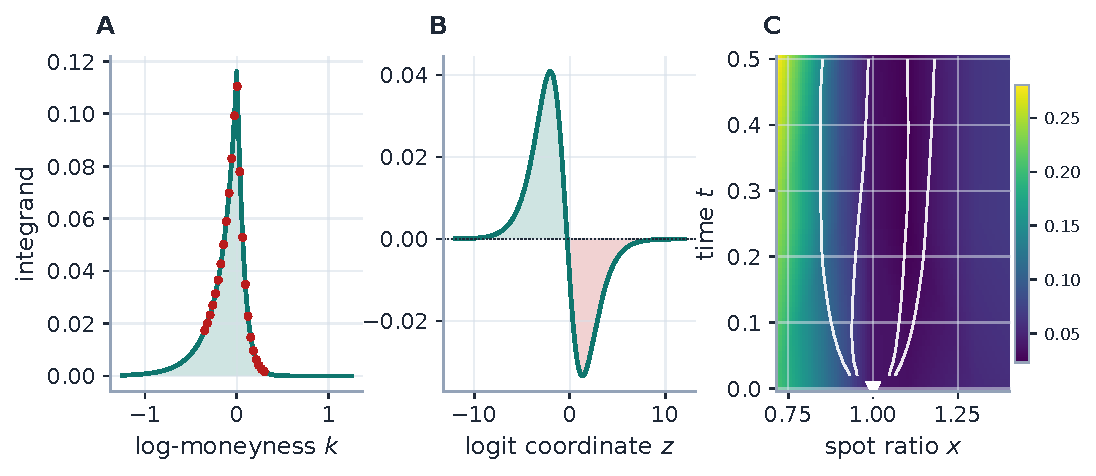
\includegraphics[width=\textwidth]{fig_vsr_three.pdf}
\caption{One number, three integrands (all panels production machinery).
A: the strike side --- the integrand of \eqref{eq:repl} on the running
LQD slice, option quotes marked; the area is $\wvs$.  B: the measure side
--- the integrand of \eqref{eq:lqd_vs} on the same slice's logit grid;
the positive left-tail lobe outweighs the negative right lobe (the
skew), and the signed area is the \emph{same} $\wvs$ to \vsragreebp\ vol
bp.  C: the generator side --- the local-variance field of the local-vol
fit to the same quotes, with occupation-measure contours
($\rho=\partial_{KK}C$ from production prices) fanning out of the spot;
the pairing $\inner{\locvar,\,\rho}$ is read off one backward solve at
the marked point $(0,1)$, and matches that surface's own strike-side
value to \vsrlvagreebp\ variance bp.}
\label{fig:three}
\end{figure}

\begin{heuristic}
Where is the number linear?  In the terminal law $\mu$, in the option
prices $C(K)$, and in the quantile $Q$ --- three linear pairings.  It is
\emph{not} linear in the implied-variance curve $\tvar(k)$: the smile
enters \eqref{eq:repl} through the nonlinear map
$\tvar\mapsto\Black(\cdot,\tvar)$.  This is worth internalizing, because
it predicts the whole cost story of \cref{sec:loop}: a model
parametrized in a chart where the pairing is linear (LQD: $Q$ is linear
in its coefficients) gets the number and its gradient at one quadrature;
a model living in the nonlinear chart pays for the coordinate change ---
per point, per parameter, per iteration.
\end{heuristic}

\paragraph{Exercise 1.}
Take a flat smile, $\tvar(k)\equiv\tvar_0$.  Show directly from
\eqref{eq:repl} --- without invoking \eqref{eq:logcontract} --- that
$\wvs=\tvar_0$.  (Hint: run the spanning proof backwards: the integral
is $\E[-2\log S_T]$ for the lognormal law with variance $\tvar_0$, and
$\E[\log S_T]=-\tvar_0/2$ by the martingale normalization.)  Conclude
that for a flat smile the fair var-swap vol equals the implied vol
exactly --- so everything a var-swap quote adds beyond the ATM level is a
statement about \emph{curvature and wings}.

%======================================================================
\section{Where the number lives}
\label{sec:lives}

Whose opinion is $\wvs$?  \Cref{fig:mass}A integrates the strike-side
integrand cumulatively across the running slice: \vsratmsharepct\% of the
number accrues within $|k|\le0.10$ --- the belly the quotes nail --- but
\vsrwingsharepct\% accrues \emph{outside the entire quoted range}, where
the smile is pure extrapolation.  That residual share is the
identifiability gap of \cref{fig:ident} made quantitative: the
\vsrlvgapbp-bp disagreement between two models fitted to the same
quotes lives almost entirely in that unquoted \vsrwingsharepct\%.  A
var-swap quote is the market pricing exactly the piece the option board
cannot.

\begin{heuristic}
Think of the var-swap quote as one very reliable \emph{wing quote}.
Liquid options cluster near the money, where they say little about the
tails; the var-swap is a traded instrument whose value loads on the
$1/K^{2}$-weighted wings.  Adding it to the objective is the cheapest way
to discipline the extrapolation the option quotes leave free ---
complementary to the Lee wing control of Note~09, which constrains the
wing \emph{slope} while the var-swap constrains the wing \emph{mass}.
The extrapolated-region machinery of Notes~09/10 polices the same
territory for arbitrage; this note's quote prices it.
\end{heuristic}

Two sanity checks calibrate the intuition.  First, the share is a
statement about the \emph{smile's} wings, not about deep-OTM dollar
prices: the $e^{-k}$ weight in \eqref{eq:repl} decays, but the Black
prices it multiplies decay much faster, so the integrand
(\cref{fig:three}A) peaks at the money --- the wings matter through
their \emph{width}, tens of percent of strike space each side,
not through any single strike.  Second, by Exercise~1 the quote adds
nothing on a flat smile; its information content scales with skew.  On
the real SPY surface of \cref{sec:hero} the published fair strikes sit up
to \vsrherospreadbp\ vol bp above the ATM vol --- that spread \emph{is}
the priced wing mass.

%======================================================================
\section{Evaluating the pairing inside the optimizer}
\label{sec:loop}

A quote is only useful if the model's own fair strike can be compared to
it at every optimizer iteration --- and differentiated.  This section is
the numerical heart of the lecture: what each representation costs, what
the production grid's error actually is (and where it comes from), and
the audit trail for each route.

\subsection{The replication as a quadrature, and its error budget}
\label{sec:budget}

Production evaluates \eqref{eq:repl} by a trapezoid on
$k\in[-H,H]$ with $H=\vsrhalfwidth$ and \vsrpoints\ points; the listing
is verbatim in structure and matches production to floating-point
identity ($10^{\vsrrefagree}$, \cref{app:ref}):

\begin{lstlisting}[caption={The strike-side quadrature of \eqref{eq:repl}
(distilled from \texttt{calib/varswap.py}; verified identical to
production).},label={lst:repl}]
def varswap_total_variance(implied_w, half=6.0, points=801):
    k = np.linspace(-half, half, points)
    w = np.maximum(implied_w(k), 1e-12)          # total-variance floor
    integ = black_call(k, w) * np.exp(-k)        # OTM call leg
    put = k < 0
    integ[put] += 1 - np.exp(-k[put])            # (e^k - 1) e^{-k}, put side
    return 2.0 * np.trapezoid(integ, k)
\end{lstlisting}

Two numerical parameters, two error terms, and it pays to know which one
is binding.  \Cref{fig:mass}B measures both against the \emph{exact}
value (the closed form of \cref{prop:quantile} on the same slice --- the
first dividend of having two representations: one audits the other).
Sweeping the half-width at a fixed fine spacing isolates
\emph{truncation}: the tails are exhausted by $H\approx\vsrtruncplateau$,
and beyond the production half-width they contribute \vsrtruncsixbp\ vol
bp --- the integrand of \cref{fig:three}A is dead there.  Sweeping $H$
at the production point count instead lets the spacing
$\Delta k=2H/(\text{\vsrpoints}-1)$ grow, and the error \emph{rises}
--- $O(\Delta k^{2})$, the trapezoid's curvature term, doubling as
$H^{2}$: \vsragreebp\ bp at $H=6$, \vsrprodeightbp\ bp at $H=8$ (ratio
$(8/6)^2$).  The production setting's \vsragreebp-bp bias is therefore
\emph{spacing}, not tails: refining to the $4001$-point diagnostics grid
at the same $H$ collapses it to \vsrreplfinebp\ bp.  Widening $H$
``to be safe'' at fixed points would make the estimate strictly worse.

\begin{figure}[H]
\centering
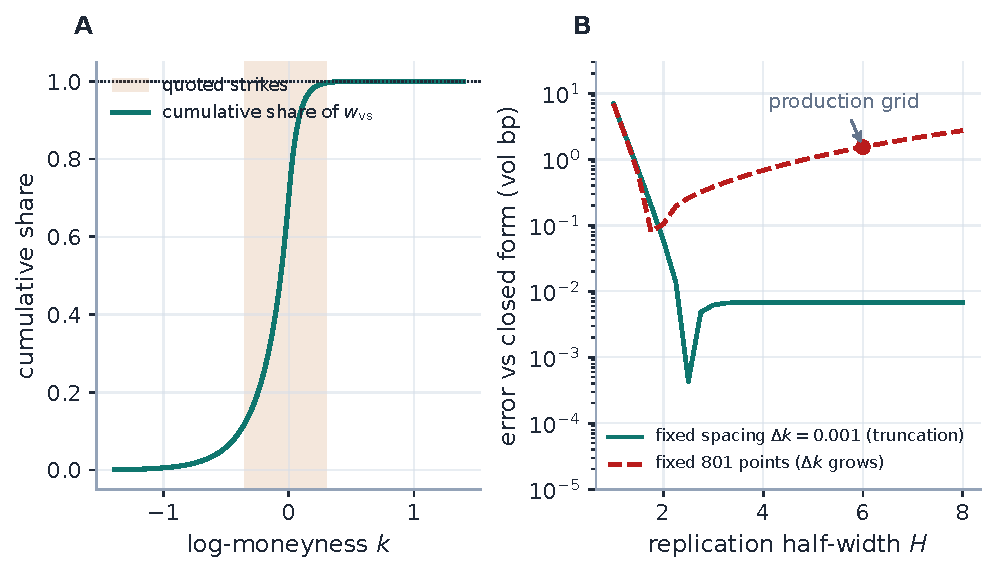
\includegraphics[width=\textwidth]{fig_vsr_mass.pdf}
\caption{Where the number lives, and what the quadrature costs.  A: the
cumulative share of $\wvs$ across strikes on the running slice ---
\vsratmsharepct\% accrues in $|k|\le0.10$, but \vsrwingsharepct\%
accrues outside the quoted band entirely (shaded): the var-swap prices
the extrapolated region.  B: the replication's error budget against the
exact closed form.  At fixed fine spacing (teal) the error is pure
truncation, exhausted by $H\approx\vsrtruncplateau$ (the mid-sweep cusp
is a sign change: left- and right-tail truncation errors briefly cancel).
At the production point count (rust, dashed) the spacing grows with $H$
and the $O(\Delta k^{2})$ trapezoid term takes over, growing like
$H^{2}$.  The production grid ($H=6$, $801$ points, dot) carries
\vsragreebp\ bp --- all spacing, no tails.}
\label{fig:mass}
\end{figure}

Why tolerate \vsragreebp\ bp in the loop at all?  Because the quadrature
runs at \emph{every objective evaluation} for the models that use it,
and a $5\times$ finer grid is $5\times$ the Black arithmetic in the
innermost loop for an error already far below quote noise and the
penalty's tolerance; the display and diagnostics path uses the
$4001$-point twin of the same integrand.  The floor on $\tvar$ in the
listing guards the inversion-free models' wings, where an extrapolated
curve could otherwise cross zero.

\subsection{The chart mismatch, as a production incident}

\begin{example}[title={Case file: the fit that took minutes}]
\textbf{Setup.}  The first wiring of the var-swap penalty used the
generic replication \eqref{eq:repl} for every model --- correct, uniform,
and apparently innocent: the integral is just a trapezoid.

\textbf{Failure mode.}  LQD fits with a var-swap target went from
milliseconds to \emph{minutes} --- a $158$-second fit was measured ---
hanging the calibrate loop.

\textbf{Diagnosis.}  The replication consumes $\tvar(k)$ on $801$
points.  LQD does not \emph{have} $\tvar(k)$: it has prices, so each
point is a Black \emph{inversion} of a quadrature-priced call --- the
nonlinear chart of the Heuristic in \cref{sec:three}.  Inside a
finite-difference Jacobian that is $801$ root-finds per parameter column
per iteration: for a nine-parameter slice, tens of thousands of
inversions per iteration to price one number the model knows in closed
form.

\textbf{Fix.}  Route each model through the representation of
\eqref{eq:master} native to its chart (\cref{sec:routes}): LQD prices
the log contract as $-2\,\E[X]$ on its existing quantile grid; SVI and
MCS keep the replication because their $\tvar(k)$ is arithmetic
(evaluated, never solved); the local-vol surface gets the source PDE
with analytic sensitivities.

\textbf{Verdict.}  The closed form agrees with the replication to
\vsragreebp\ vol bp (each validating the other), and the var-swap
penalty now costs essentially nothing in any model.  \emph{A uniform
implementation is not a virtue when the models' native objects differ
--- evaluate a shared functional in each model's own coordinates.}
\end{example}

\subsection{The three routes, costed}
\label{sec:routes}

\textbf{LQD: the quantile side, one trapezoid.}  The slice's standing
grid already carries $Q(z)$ and $u(1-u)=\Lo(1-\Lo)$, so
\eqref{eq:lqd_vs} is one dot product over the grid --- $O(n)$ with no
new function evaluations (\cref{app:ref} gives the two-line
implementation).  Linearity pays twice: $Q$ is linear in the slice's
coefficients, so $\partial\wvs/\partial\theta_\ell$ is the \emph{same}
quadrature applied to the basis responses --- no extra solves.

\textbf{SVI and MCS: the strike side, arithmetic.}  For SVI (a
hyperbola, Note~02) and Multi-Core Sigmoid (a log-cosh sum, Note~03) the
total variance $\tvar(k)$ is closed-form arithmetic, so
\cref{lst:repl} is $801$ arithmetic evaluations --- no inversion,
negligible against the data residuals.  These models were never the
problem; the case file's trap was applying their route to a model in
the other chart.

\textbf{Local volatility: the generator side, one backward sweep.}  The
production discretization of \eqref{eq:source_pde} reuses the forward
Dupire march's machinery wholesale: the same $\half\locvar x^{2}
\partial_{xx}$ stencil, the same implicit-Euler tridiagonal factor per
step, marched backward from $g(T,\cdot)=0$ with $+\locvar$ as source; at
the degenerate boundaries $x^2\partial_{xx}\to0$ and the rows reduce to
pure accumulation $g\mathrel{+}=\Delta t\,\locvar$.  The number is read
at the grid node $x=1$ (enforced to be one).  Sensitivities come from
the same factorization: differentiating the marched system in
$\theta_\ell$ yields companion problems with source
$\half\phi_\ell x^{2}\partial_{xx}g+\phi_\ell$ ($\phi_\ell$ the affine
basis), solved as extra right-hand sides against the already-factored
operator --- the multi-RHS pattern of Note~04's forward sweep.  When a
var-swap quote frees the left-wing extrapolation slope
(\cref{sec:limits}), one more column prices its sensitivity.

\Cref{fig:audit} is the route's audit.  Panel A compares every analytic
$\partial \wvs/\partial\theta_\ell$ against central finite differences:
agreement to \vsrsensabs\ absolute across sensitivities spanning four
orders of magnitude --- relative error \vsrsensrel\ on the
\vsrsenslive\ of \vsrsenstotal\ parameters the horizon actually sees
(the two excluded are far-wing corners of the initial time row, whose
true sensitivity is $\sim10^{-11}$: no path mass ever visits them).
Panel B closes the loop between representations: across horizons, the
backward solve's $g(0,1)$ tracks the surface's own strike-side
replication within \vsrlvagreebp\ variance bp --- two discretizations of
two different integrals in \eqref{eq:master}, agreeing because the
mathematics says they must.

\begin{figure}[H]
\centering
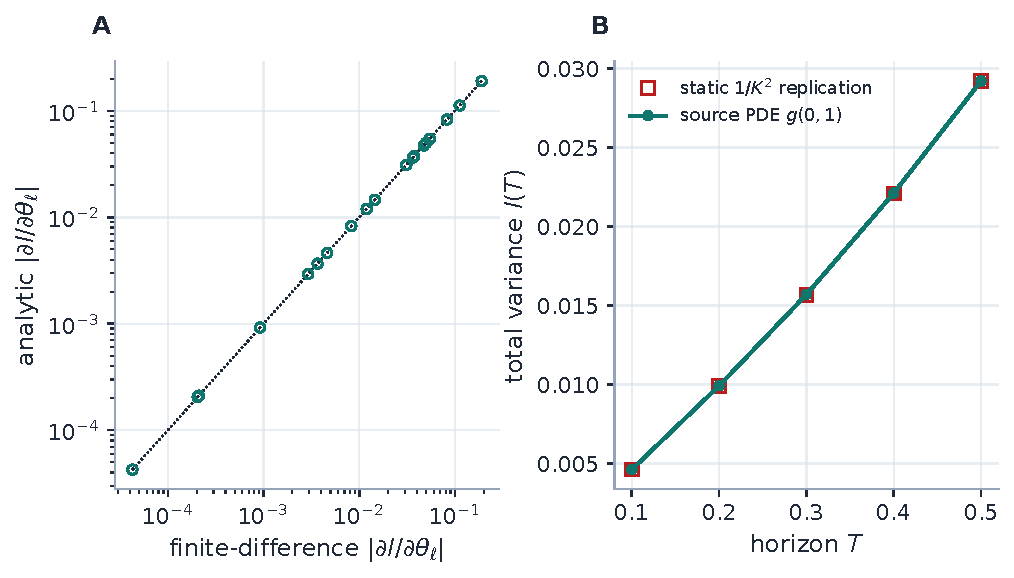
\includegraphics[width=\textwidth]{fig_vsr_audit.pdf}
\caption{The generator-side route, audited (production local-vol
machinery).  A: analytic sensitivities $\partial\wvs/\partial
\theta_\ell$ from the multi-RHS backward solve against central finite
differences --- on the diagonal to \vsrsensabs\ across four decades;
the two parameters with no path mass under this horizon are omitted.
B: the source PDE's $g(0,1)$ against the same surface's static
$1/K^{2}$ replication across horizons --- two representations of
\eqref{eq:master}, within \vsrlvagreebp\ variance bp at every $T$.}
\label{fig:audit}
\end{figure}

\begin{perfbox}
Cost accounting per objective evaluation, $n$ grid points, $m$
parameters: LQD closed form $O(n)$ with gradient by linearity (free);
SVI/MCS replication $O(\text{\vsrpoints})$ arithmetic; LV source PDE one
backward sweep $\approx$ one extra value solve, plus $m$ extra
right-hand sides on factored tridiagonal systems ($O(n_x m)$ per step)
for the full gradient.  The route that was retired --- replication over
an inversion-priced smile --- was $O(\text{\vsrpoints})$ root-finds per
Jacobian \emph{column}: the measured $158$-second fit.  What remains
deliberately unoptimized: with a var-swap target the parametric models
currently switch to a finite-difference Jacobian for the whole residual
stack (each column re-evaluates a cheap closed form, so the cost is
benign); wiring the var-swap row into the analytic Jacobian is deferred
work (\cref{app:perf}).
\end{perfbox}

\paragraph{Exercise 2.}
The measure-side integrand decays like $|z|e^{-|z|}$ (exponential tails
make $Q$ asymptotically linear in $z$; the logistic weight supplies
$e^{-|z|}$).  Bound the truncation error of \eqref{eq:lqd_vs} beyond the
standing grid's half-width $z_{\max}=40$ by
$\int_{40}^{\infty}ze^{-z}\dd z=41\,e^{-40}$, and evaluate it.  Compare
with double-precision machine epsilon, and with the strike-side
truncation error at $H=6$ from \cref{fig:mass}B (\vsrtruncsixbp\ vol
bp): both representations truncate infinite integrals, but the measure
side's grid was built once for \emph{pricing}, and the var-swap rides it
for free.

%======================================================================
\section{The quote as one more residual}
\label{sec:penalty}

The pairing priced, the quote must now \emph{act} on the fit.  Both are
stated in volatility --- $\svs=\sqrt{\wvs/T}$ --- and the target enters
every parametric model's least-squares stack as a single extra residual,
\begin{equation}
r_{\mathrm{vs}}
=\sqrt{\lam_{\mathrm{vs}}}\,
\big(\svs^{\mathrm{model}}-\svs^{\mathrm{quote}}\big),
\qquad
\lam_{\mathrm{vs}}=p\sum_i\lam_i ,
\label{eq:resid}
\end{equation}
with $p$ the declared fraction (default ten percent) of the node's
summed option-quote weight.  Three design decisions, each doing quiet
work:

\emph{Vol units.}  The data residuals are vol-metric for every model ---
natively for SVI/MCS, via the vega-normalized dictionary of Note~07 for
LQD/LV --- so \eqref{eq:resid} stacks onto them without a hidden
exchange rate; a one-vol-point var-swap miss trades against a
one-vol-point quote miss at the declared ratio and nothing else.

\emph{A relative weight.}  An absolute weight would mean something
different on every node; $\lam_{\mathrm{vs}}=p\sum\lam_i$ makes the
quote carry a declared \emph{share} of the objective whether the node
has ten quotes or a hundred (invariant~4) --- the same normalization
philosophy as Note~07's mean-one weights, applied to a functional
observation.

\emph{A soft target.}  \eqref{eq:resid} is a pull, not a constraint: the
quote bargains with the option quotes at strength $p$.

The local-vol calibrator states the same trade in its own residual
space.  Its var-swap rows live in total variance, so the vol-space
weight must be converted: a tolerance of one vol point corresponds, by
$\partial\wvs/\partial\svs=2\svs T$, to a total-variance tolerance
$\zeta=2\svs T\times0.01/\sqrt{\lam_{\mathrm{vs}}}$, and the residual
$(\wvs^{\mathrm{model}}-\wvs^{\mathrm{quote}})/\zeta$ then squares to
exactly the weight of \eqref{eq:resid} --- one functional, one weight
semantics, two coordinate systems.

\subsection{The dial, and a worked pull}

\Cref{fig:dial} sweeps the fraction $p$ against a quote pitched
$1.5$ vol points above the running slice's natural \vsrclosed\%: the
fitted fair strike rises monotonically toward the quote --- the pull is
a continuous dial, not a switch --- reaching \vsrpulled\% at the shipped
default ($p=10\%$): \vsrpullsharepct\% of the gap.

\begin{figure}[H]
\centering
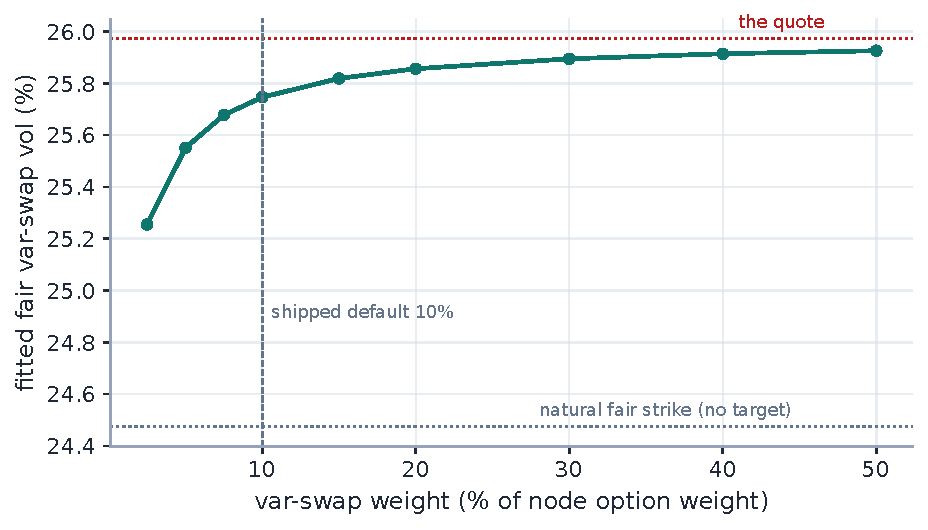
\includegraphics[width=0.80\textwidth]{fig_vsr_dial.pdf}
\caption{The relative-weight dial (production fits at every point).  A
var-swap quote $1.5$ vol points above the smile's natural fair strike
pulls the fitted fair strike monotonically toward it as the declared
weight fraction grows; at the shipped default of ten percent the fit
concedes \vsrpullsharepct\% of the gap.  The quote bargains --- it does
not dictate.}
\label{fig:dial}
\end{figure}

\Cref{fig:pull} shows \emph{how} the smile pays for the pull at the
default weight.  Panel A: the targeted fit steepens both wings while
still threading the quotes --- the worst option-quote concession is
\vsrpullfitbp\ vol bp (against \vsrbasefitbp\ bp for the untargeted
fit): visible, bounded, and exactly the bargain $p=10\%$ declares.
Panel B looks underneath, at the risk-neutral density: the extra
variance is bought with tail mass on both sides, the belly barely
moving --- the var-swap target edits precisely the region the option
quotes do not own (\cref{sec:lives}).  \Cref{tab:vs} collects the
numbers.

\begin{figure}[H]
\centering
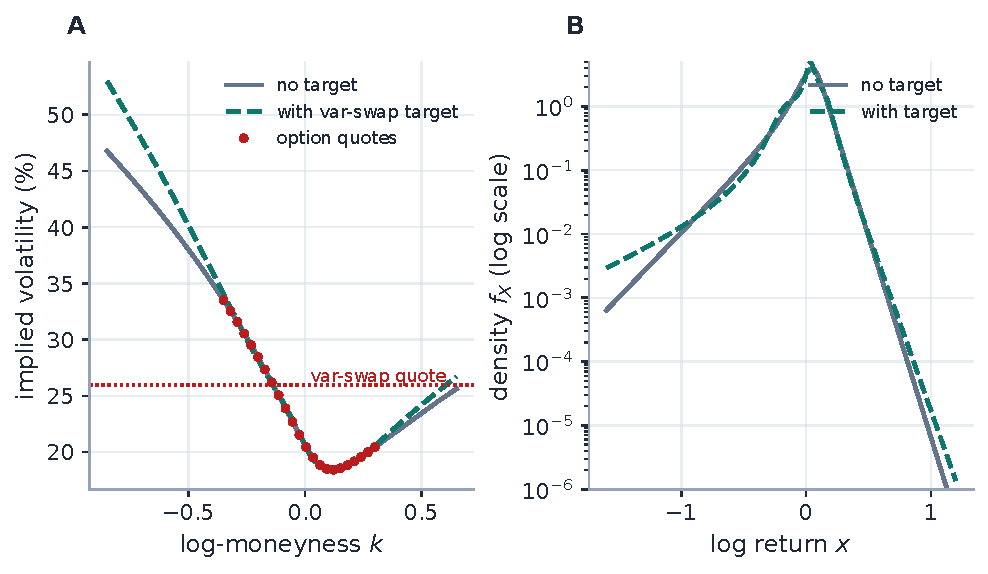
\includegraphics[width=\textwidth]{fig_vsr_pull.pdf}
\caption{Anatomy of a pull (running slice; quote \vsrtarget\%, default
weight).  A: the targeted fit (dashed) lifts its fair strike from
\vsrclosed\% to \vsrpulled\% by steepening the wings, conceding at most
\vsrpullfitbp\ vol bp at any option quote.  B: the same two fits as
densities (log scale): the added variance is wing mass --- both tails
fatten while the belly, where the quotes live, is untouched.  The target
spends its budget exactly where \cref{fig:mass}A said the number
lives.}
\label{fig:pull}
\end{figure}

\begin{table}[H]
\centering
\caption{The worked pull (fresh production run): the two exact
representations on the untargeted slice, and the targeted refit at the
default weight.}
\label{tab:vs}
\begin{tabular}{lr}
\toprule
Quantity & Value\\
\midrule
Natural fair var-swap vol (closed form \eqref{eq:lqd_vs}) & $\vsrclosed\%$\\
Same slice by strike-side replication \eqref{eq:repl} & $\vsrrepl\%$\\
Representation agreement & $\vsragreebp$ vol bp\\
Var-swap quote (target) & $\vsrtarget\%$\\
Targeted fit's fair var-swap vol & $\vsrpulled\%$\\
Share of the gap conceded & $\vsrpullsharepct\%$\\
Worst option-quote concession & $\vsrpullfitbp$ vol bp\\
\bottomrule
\end{tabular}
\end{table}

\paragraph{Exercise 3.}
Model the fit's resistance as one effective stiffness: near the optimum
the fitted fair vol solves
$\svs=\svs^{\mathrm{nat}}+\frac{\lam_{\mathrm{vs}}}
{\lam_{\mathrm{vs}}+\kappa}\big(\svs^{\mathrm{quote}}
-\svs^{\mathrm{nat}}\big)$ for some $\kappa$ summarizing how strongly
the data-plus-ridge terms resist a wing steepening.  Calibrate $\kappa$
from the default point of \cref{fig:dial}
($\lam_{\mathrm{vs}}=0.10\times23=2.3$, conceded share
\vsrpullsharepct\%), then predict the conceded share at $p=2.5\%$ and
compare with the figure.  The one-parameter model tracks the whole dial
to a few points of share --- the pull really is a scalar bargain.

%======================================================================
\section{The real object}
\label{sec:hero}

\Cref{fig:hero} leaves the running example for the application's own
output: a live SPY surface (Massive feed, \vsrheronodes\ expiries,
valuation date 2026-07-18), fitted in production with a
twelve-parameter slice per expiry.  The teal curve is the fair var-swap
vol the application \emph{publishes} per node; the crosses re-derive
each one by \cref{prop:quantile}'s closed form from the stored slice
parameters --- agreement \vsrheroagreebp\ vol bp, an end-to-end audit
that the shipped number is the mathematics of this note and nothing
else.  The var-swap vol rides above the ATM vol at every expiry, by up
to \vsrherospreadbp\ vol bp at the long end: the skew's wing mass,
priced (\cref{sec:lives}); the term structure of that spread is itself a
tradeable object, and the calendar machinery of Note~11 consumes these
per-node strikes.

\begin{figure}[H]
\centering
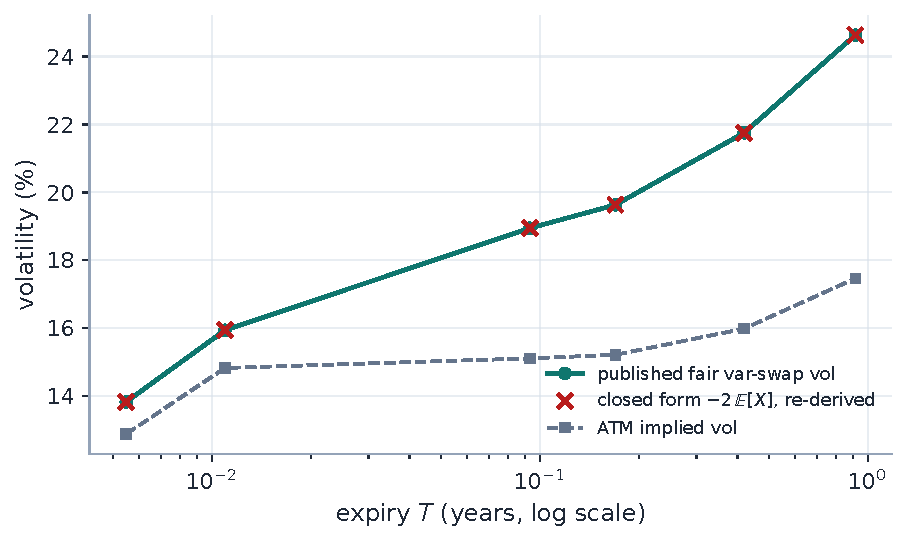
\includegraphics[width=0.86\textwidth]{fig_vsr_hero.pdf}
\caption{The real object: a live SPY surface's published fair var-swap
vols across \vsrheronodes\ expiries (teal), re-derived from the stored
slice parameters by the closed form \eqref{eq:lqd_vs} (crosses) ---
agreement \vsrheroagreebp\ vol bp.  The fair strike sits above the ATM
vol (dashed) everywhere, by up to \vsrherospreadbp\ vol bp at the long
end: the skew's wing mass is priced into the swap, and the spread grows
with the skew's room to act.}
\label{fig:hero}
\end{figure}

Operationally the quote is a first-class citizen of the smile session:
one scalar per node (invariant~1), shared verbatim by the parametric and
local-vol views, settable, excludable and removable with a hundred-deep
undo/redo history kept separate from the option-quote edits, versioned
so an edit refits exactly once, and serialized with the workspace.
Setting the feature off, or the node having no quote, reproduces the
untargeted fit byte for byte (invariant~2) --- the smile payload also
carries the model's own fair strike when no quote is set, so the desk
can seed a quote \emph{at} the model before nudging it.  A companion
prior-side target reuses the same residual machinery to hold a fit near
its prior's fair strike under the persistence framework of Note~13.

%======================================================================
\section{What is genuinely original here}
\label{sec:original}

The spanning identity is Carr--Madan; the quantile representation of a
mean and Feynman--Kac are classical.  The contributions are practical
and, in one case, a small piece of numerical epistemology:
\begin{enumerate}[leftmargin=1.6em]
\item the \emph{per-model routing} of one functional through three
representations \eqref{eq:master} --- closed form for the quantile-chart
model, arithmetic replication for the vol-chart models, a source PDE
with multi-RHS analytic sensitivities for the generator-chart model ---
which is what makes a var-swap target affordable \emph{inside} the
optimizer loop rather than as a post-hoc check;
\item the \emph{relative weighting} of a functional observation
\eqref{eq:resid}, keeping the quote's share of the objective declared
and node-independent, with the exact vol-to-variance weight conversion
for the local-vol residual space;
\item the \emph{cross-representation audit discipline}: every route is
checked against a mathematically distinct route of the same number
(closed form vs replication at \vsragreebp\ bp; source PDE vs static at
\vsrlvagreebp\ variance bp; published app values vs re-derivation at
\vsrheroagreebp\ bp) --- representations are cheap redundancy, and
redundancy is how a pricing library audits itself.
\end{enumerate}

%======================================================================
\section{Limitations}
\label{sec:limits}

Where the guarantees stop.  \emph{The diffusion assumption is load-bearing}:
\eqref{eq:ito} uses It\^o on a continuous path, and under jumps the
realized-variance/log-contract equivalence acquires a cubic correction:
a jump of relative size $J$ contributes
$2[J-\log(1+J)]-\log^{2}(1+J)=\tfrac13J^{3}+O(J^{4})$ to the gap between
the replicated and realized strikes, so for jumpy underliers the quote
and the replication price subtly different things --- the models here
fit the \emph{diffusion} fair strike.  Discrete cash dividends sit outside the clean
forward-normalized derivation for the same reason.  \emph{The number
inherits the model's extrapolation}: \vsrwingsharepct\% of it lives
beyond the quoted strikes (\cref{fig:mass}A), so a var-swap-targeted fit
is only as meaningful as the wing behaviour of the model absorbing it
--- indeed on the local-vol surface a var-swap quote deliberately
\emph{frees} the left-wing extrapolation slope so the target has a wing
lever to act on; the fitted slope is then an inference, not an
observation.  \emph{The strike-side quadrature carries a measured
$O(\Delta k^{2})$ bias} (\vsragreebp\ bp at production settings,
\cref{sec:budget}) --- far below quote noise, but a bias with a sign,
and the error budget shows widening $H$ without refining $\Delta k$
worsens it.  \emph{The penalty is a pull, not a constraint}: at the
default weight the fit concedes \vsrpullsharepct\% of a $1.5$-point gap
(\cref{fig:dial}); a desk wanting the quote hit exactly must say so
through the weight, and accept the option-side concessions of
\cref{fig:pull}A.  \emph{Provenance is the user's problem}: var-swap
quotes are OTC marks, not exchange prints; the machinery applies
whatever level is set, one per node, with no staleness screen of its
own.  And the parametric models' Jacobian falls back to finite
differences when a target is active --- cheap here, but a deliberate,
documented deferral (\cref{app:perf}).

\appendix
%======================================================================
\section{Hyperparameter atlas}
\label{app:atlas}

The only home for settings names: the body speaks mathematics, this
table speaks configuration.

\begin{longtable}{p{0.26\textwidth}p{0.13\textwidth}p{0.53\textwidth}}
\caption{Variance-swap hyperparameters, surfaced and hidden.}
\label{tab:atlas}\\
\toprule Knob & Default & Role\\ \midrule
\endfirsthead \toprule Knob & Default & Role\\ \midrule \endhead
\multicolumn{3}{l}{\emph{Surfaced (OptionsSettings)}}\\ \midrule
\texttt{varSwapEnabled} & \texttt{true} & Master toggle (surfaces the
var-swap level in the UI); the penalty activates only when a quote is
set on the node.\\
\texttt{varSwapWeightPct} $p$ & $10\%$ & The quote's weight as a
fraction of the node's summed option weight, \eqref{eq:resid}.\\
\texttt{varSwapMethod} (LV) & \texttt{static} & Local-vol fair-strike
pricer: strike-side replication or the source PDE
\eqref{eq:source_pde}; parametric models always use their own routes.\\
\midrule
\multicolumn{3}{l}{\emph{Hidden}}\\ \midrule
\texttt{VS\_HALF\_WIDTH} $H$ & $\vsrhalfwidth$ & Replication half-width
in log-moneyness (in-loop grid).\\
\texttt{VS\_POINTS} & $\vsrpoints$ & Replication trapezoid points
(in-loop); the diagnostics/display twin uses $4001$ on the same $H$.\\
\texttt{\_W\_FLOOR} & $10^{-12}$ & Total-variance floor inside the
integrand (wing guard).\\
\texttt{\_VARSWAP\_K\_LO} (LV) & $0.01$ & Lower strike-ratio cutoff of
the LV static replication weights.\\
\texttt{\_VOL\_TOL} (LV) & $0.01$ & The one-vol-point unit in the
vol-to-variance weight conversion $\zeta$ of \cref{sec:penalty}.\\
\texttt{MAX\_UNDO\_DEPTH} & $100$ & Depth of the var-swap session's
undo/redo stacks.\\
\bottomrule
\end{longtable}

%======================================================================
\section{Performance notes}
\label{app:perf}

Protocol: timings quoted here are historical measurements from the
production incident ledger (never re-timed for this edition); accuracy
numbers are from this edition's generator, which runs the production
code on the running slice and the standing SPY export.

\begin{enumerate}[leftmargin=1.6em]
\item \textbf{Retired: generic replication for LQD.}  $801$ Black
inversions per finite-difference Jacobian column per iteration; measured
at $158$ seconds for a fit that runs in milliseconds without a target.
Replaced by the closed form \eqref{eq:lqd_vs}: one $O(n)$ quadrature on
the slice's existing grid, gradient by linearity.  The two routes agree
to \vsragreebp\ vol bp (\cref{tab:vs}).
\item \textbf{SVI/MCS replication.}  \vsrpoints\ arithmetic smile
evaluations per objective call; negligible against the data residuals.
The in-loop grid's \vsragreebp-bp $O(\Delta k^2)$ bias
(\cref{sec:budget}) is a deliberate latency/accuracy trade; the
$4001$-point diagnostics twin reads \vsrreplfinebp\ bp.
\item \textbf{LV source PDE.}  One extra backward sweep reusing the
forward march's factored tridiagonal steps; full analytic gradient via
multi-RHS at $O(n_x m)$ per step; verified against finite differences
at \vsrsensabs\ (\cref{fig:audit}A).  Basis precomputation is
$\theta$-independent and shares the forward solver's memory-budget
guard.  The static route remains the shipped default; the source PDE is
the faster alternative on fine strike grids and is truncation-free in
strike.
\item \textbf{Deferred, deliberately:} the parametric models switch to a
finite-difference Jacobian whenever a var-swap (or prior var-swap)
target is active --- each column re-evaluates only cheap closed
forms, so the observed cost is benign; wiring the target row into the
analytic Jacobians is the remaining lever, shelved until it earns its
complexity.
\end{enumerate}

%======================================================================
\section{Traceability}
\label{app:trace}

\begingroup
\small
\setlength{\tabcolsep}{4pt}
\renewcommand{\arraystretch}{1.15}
\begin{longtable}{@{}p{0.42\textwidth}p{0.10\textwidth}p{0.44\textwidth}@{}}
\caption{Claims in this note and the code/tests that lock them.}
\label{tab:trace}\\
\toprule Claim & Object & Code anchor \newline \emph{Test anchor}\\ \midrule
\endfirsthead
\toprule Claim & Object & Code anchor \newline \emph{Test anchor}\\ \midrule
\endhead
Penalty pulls every model's fair strike toward the quote &
\eqref{eq:resid} &
\nolinkurl{volfit/calib/varswap.py}\newline
\nolinkurl{tests/test_varswap.py::test_penalty_pulls_model_varswap_toward_quote_all_models}\\
\addlinespace
No target / disabled is byte-identical &
invariant~2 &
\nolinkurl{volfit/calib/varswap.py}\newline
\nolinkurl{tests/test_varswap.py::test_none_target_is_byte_identical};
\nolinkurl{::test_disabling_varswap_drops_the_penalty}\\
\addlinespace
The pull is monotone in the weight (the dial) &
\cref{fig:dial} &
\nolinkurl{volfit/calib/varswap.py}\newline
\nolinkurl{tests/test_varswap.py::test_weight_strength_monotone}\\
\addlinespace
One quote per node; set/exclude/undo/redo; validation without mutation &
invariant~1 &
\nolinkurl{volfit/api/varswap_session.py}\newline
\nolinkurl{tests/test_varswap.py::test_session_set_exclude_include_remove};
\nolinkurl{::test_session_undo_redo_and_validation}\\
\addlinespace
Payload carries the level and the model's own fair strike; endpoints
refit and undo &
\cref{sec:hero} &
\nolinkurl{volfit/api/routers/varswap.py}\newline
\nolinkurl{tests/test_varswap.py::test_smile_payload_carries_varswap};
\nolinkurl{::test_varswap_endpoints_refit_and_undo};
\nolinkurl{::test_term_reports_varswap_quote}\\
\addlinespace
The LV fit carries and honours the shared quote &
\cref{sec:routes} &
\nolinkurl{volfit/api/affine_fit.py}\newline
\nolinkurl{tests/test_varswap.py::test_affine_fit_carries_and_honours_varswap}\\
\addlinespace
Source PDE matches static; analytic sensitivities match FD; both
methods hit quotes &
\eqref{eq:source_pde} &
\nolinkurl{volfit/models/localvol/varswap_pde.py}\newline
\nolinkurl{tests/test_varswap_source.py::test_source_pde_value_matches_static};
\nolinkurl{::test_source_pde_theta_sensitivity_matches_fd};
\nolinkurl{::test_source_pde_a_sensitivity_matches_fd};
\nolinkurl{::test_calibrate_source_pde_hits_varswaps}\\
\addlinespace
LQD closed form (the case-file fix) &
\eqref{eq:lqd_vs} &
\nolinkurl{volfit/models/lqd/quadrature.py}\newline
\nolinkurl{tests/test_varswap.py} (all-models pull); agreement
\vsragreebp\ bp (\cref{tab:vs}); hero audit \vsrheroagreebp\ bp
(\cref{fig:hero})\\
\bottomrule
\end{longtable}
\endgroup

%======================================================================
\section{Reference implementation: both exact routes}
\label{app:ref}

Both listings were executed against their production counterparts by
this edition's generator on every run: agreement $10^{\vsrrefagree}$
(floating-point identity).  The strike-side quadrature is
\cref{lst:repl} in the body; the measure side is two lines, because the
slice's pricing grid already carries everything the log contract needs
(the quantile $Q(z)$ and the logistic weight $u(1-u)$; the integrand
decays like $|z|e^{-|z|}$, Exercise~2):

\begin{lstlisting}[caption={The quantile-side closed form
\eqref{eq:lqd_vs}: the fair strike as the mean log-return (distilled
from \texttt{models/lqd/quadrature.py}).}]
def var_swap_strike(z, q_z, u):        # z: logit grid, q_z = Q(z), u = expit(z)
    return -2.0 * np.trapezoid(q_z * u * (1 - u), z)   # = -2 E[X]
\end{lstlisting}

\begin{thebibliography}{9}
\bibitem{Neuberger1994} A.~Neuberger.  The log contract.
\emph{J.\ Portfolio Management}, 20(2):74--80, 1994.
\bibitem{CarrMadan1998} P.~Carr and D.~Madan.  Towards a theory of
volatility trading.  In \emph{Volatility}, Risk Books, 1998.
\bibitem{DemeterfiDermanKamalZou1999} K.~Demeterfi, E.~Derman, M.~Kamal
and J.~Zou.  A guide to volatility and variance swaps.
\emph{J.\ Derivatives}, 6(4):9--32, 1999.
\bibitem{BreedenLitzenberger1978} D.~Breeden and R.~Litzenberger.
Prices of state-contingent claims implicit in option prices.
\emph{J.\ Business}, 51(4):621--651, 1978.
\bibitem{Gatheral2006} J.~Gatheral.  \emph{The Volatility Surface}.
Wiley, 2006.
\end{thebibliography}

\end{document}
